\providecommand{\rasd}{..}
\documentclass[../RASD.tex]{subfiles}

\begin{document}
    \chapter{Architectural Design}\label{ch:architectural-design}
    \section{Overview}\label{sec:overview}
    From an external point of view, users using their smartphones, exploits the different services offered by SafeStreets that are different for citizen and authority.

    The application to be developed is based on one application component ( application logic) which manages the interactions between different components of the system.

    Application logic is present both in the mobile view and in the back-end logic. In mobile view there is the management of the GUI and of the connection with other useful components present in the smartphone: GPS and camera; while in the back-end logic there is the most of the logic and also the interfaces to external services: Database provider, Plate recognition provider, map provider and authentication provider.
    \begin{figure}[H]
        \centering
        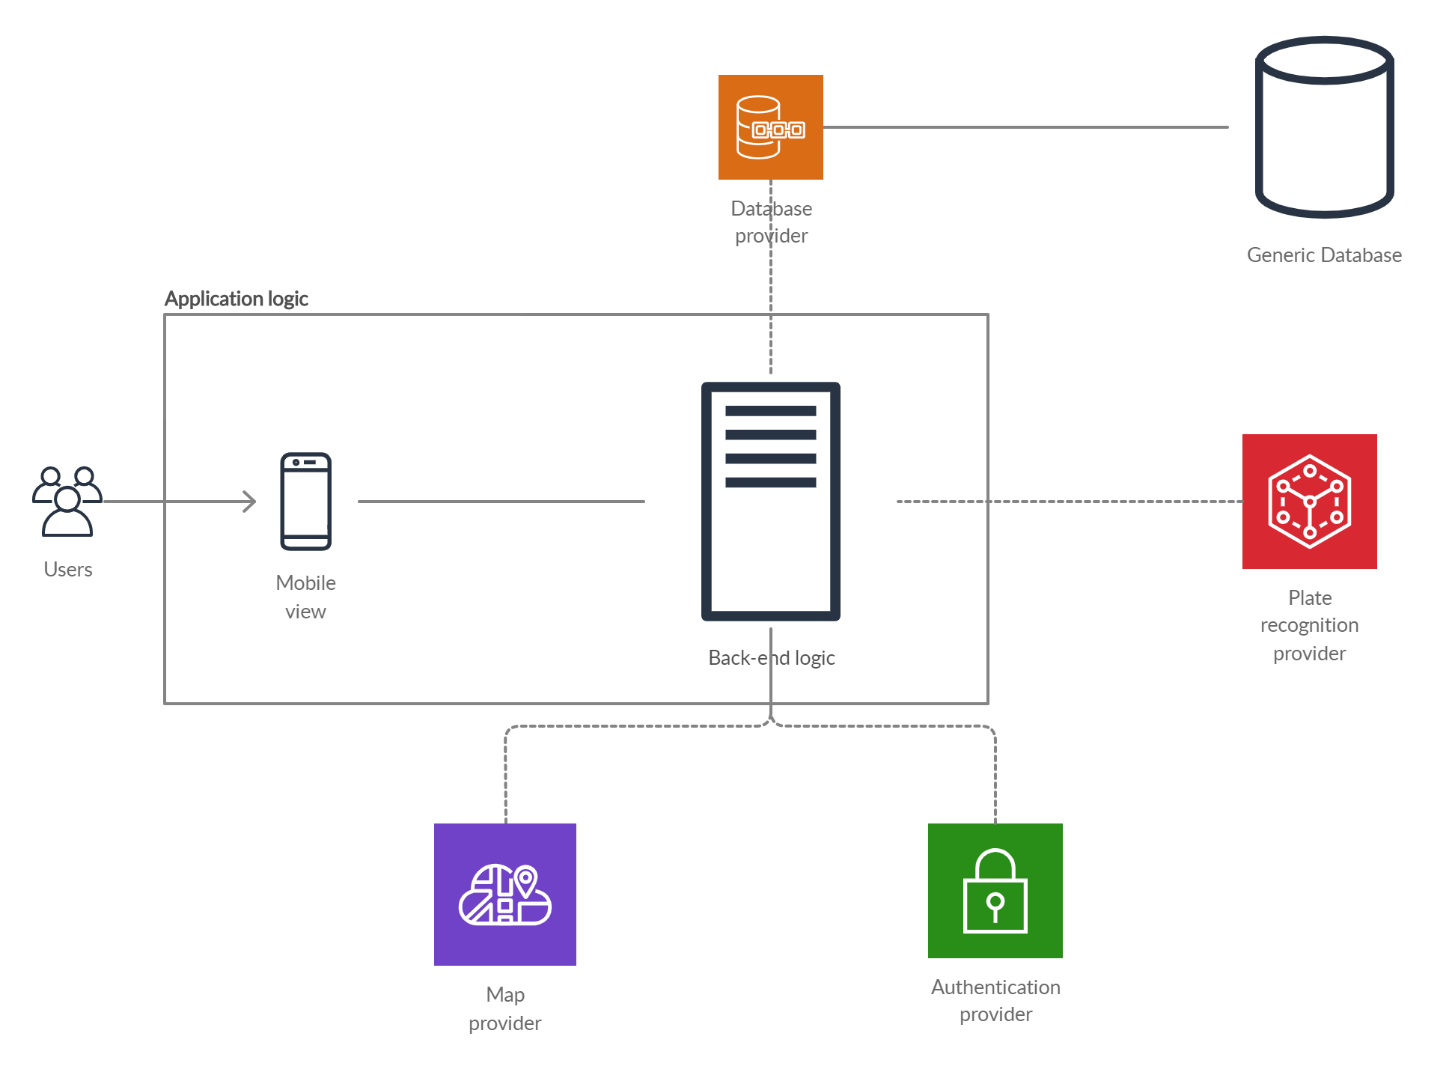
\includegraphics[scale = 1]{assets/overview.png}\\[1.6 cm]
        \caption[\textit{OverView} Diagram]{Overview diagram of the application.}
    \end{figure}
    \section{Component View}\label{sec:component-view}
    \begin{figure}[H]
        \centering
        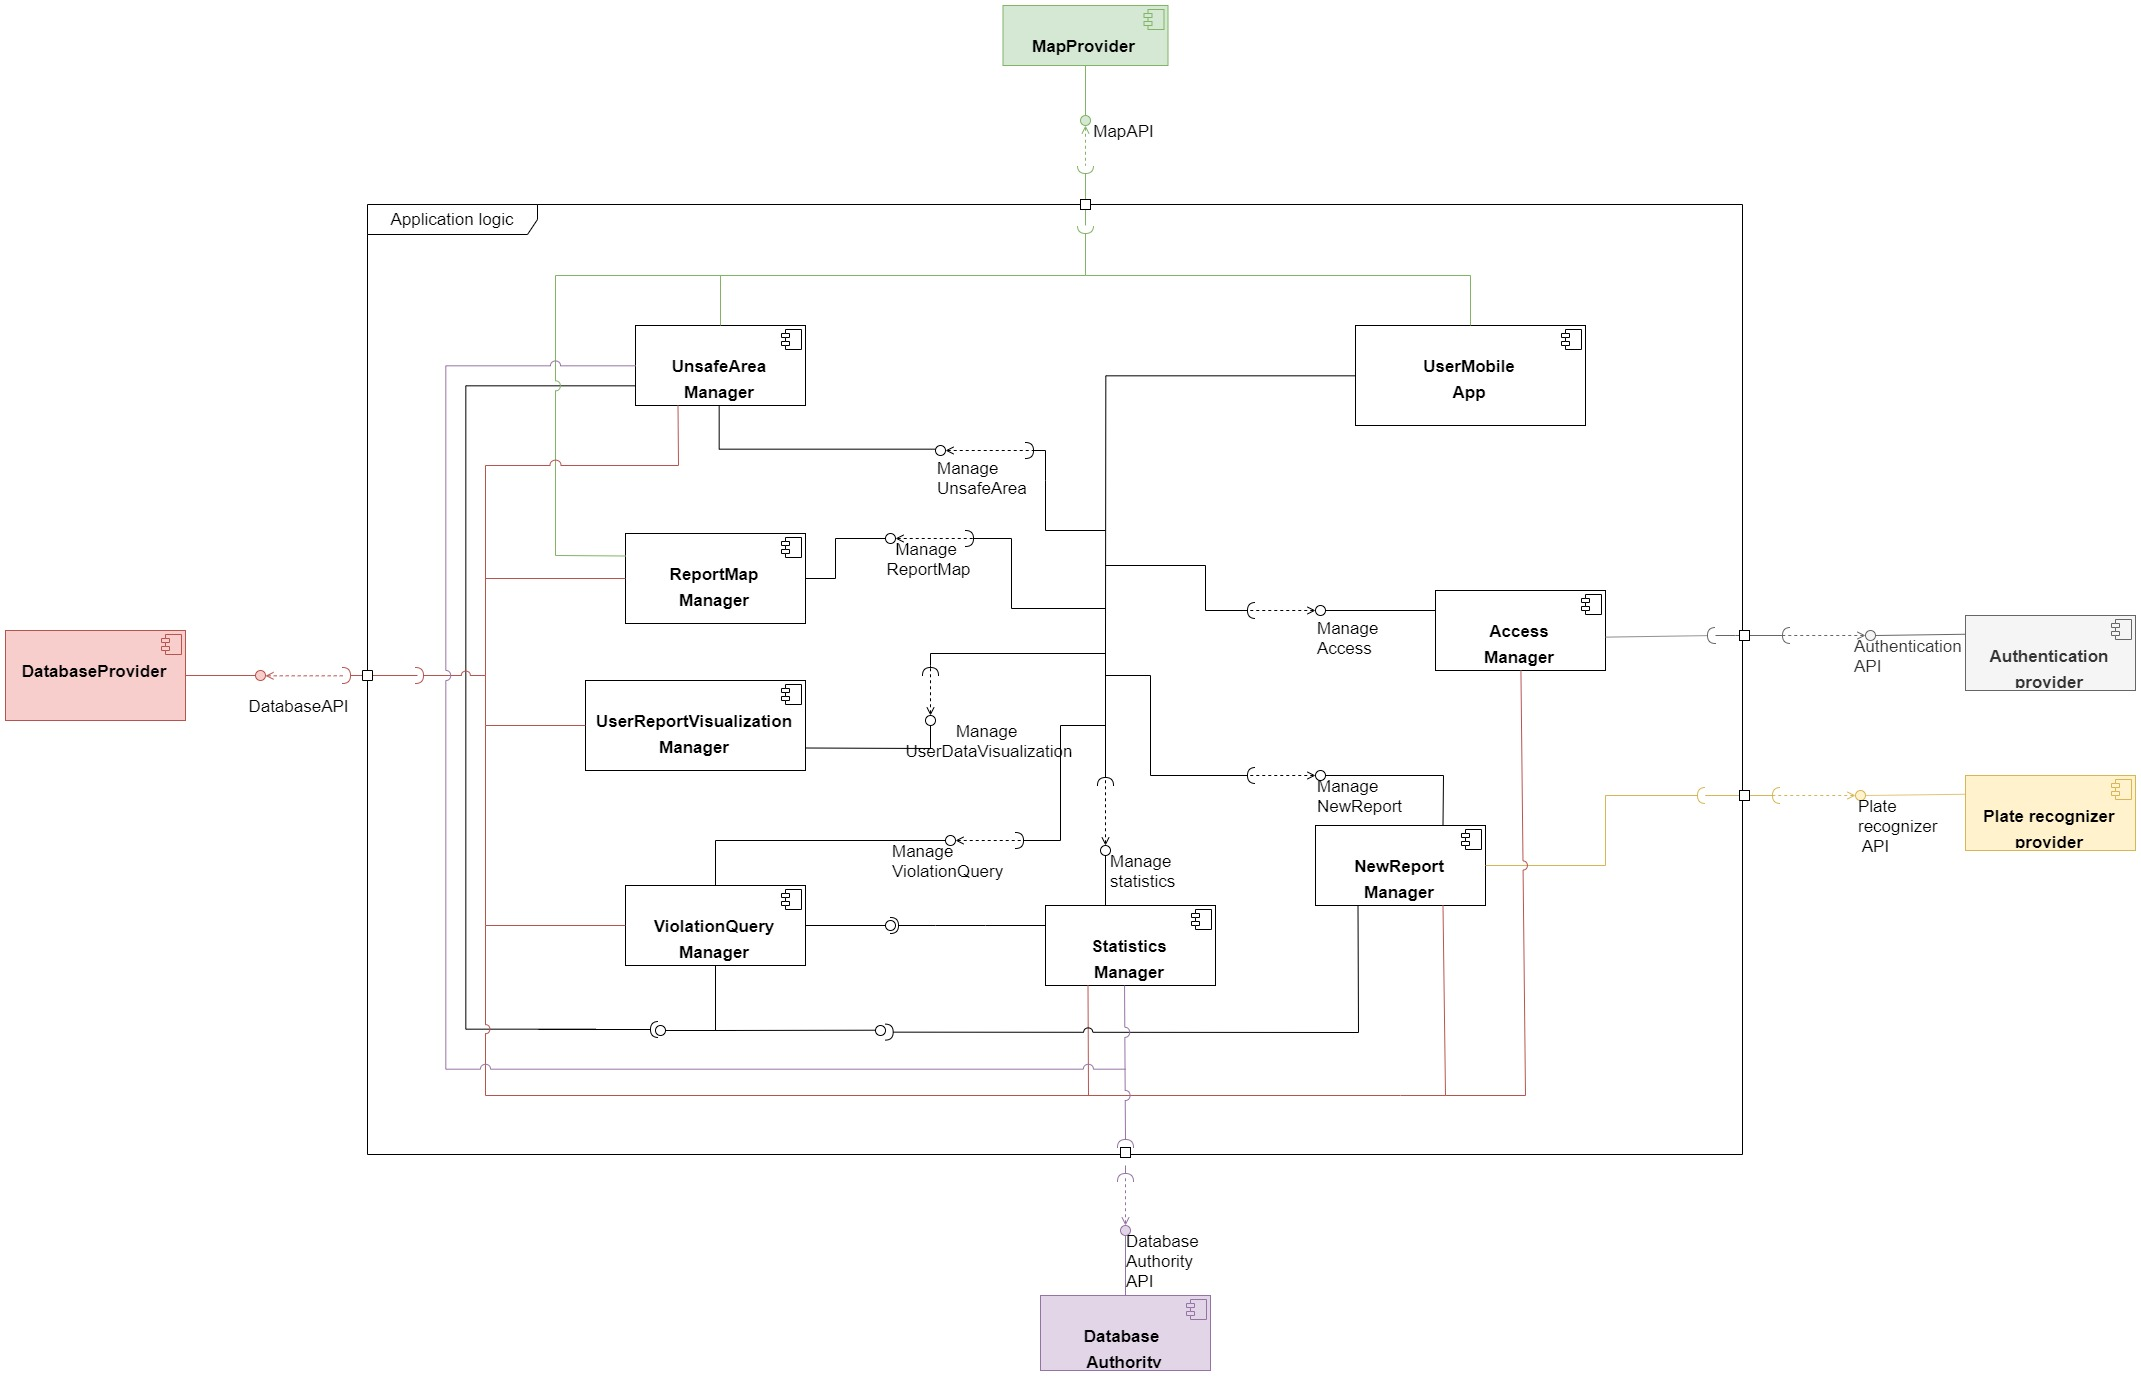
\includegraphics[scale = 1]{assets/component.png}\\[1.6 cm]
        \caption[\textit{Component} Diagram]{Component diagram of the application.}
    \end{figure}
    The components’ functions contained in the application are described in the following:

\end{document}